% The parabola V(y-x^2); the x-axis and the origin are highlighted.
% Source: book/tex/alg-geom/affine-var.tex (§ Coordinate rings).
\documentclass[border=2mm]{standalone}
\usepackage{tikz}\usepackage{amssymb}
\begin{document}
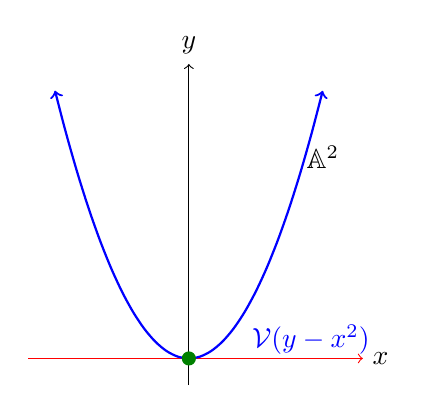
\begin{tikzpicture}[scale=0.85]
  \draw[red,->] (-2.4,0) -- (2.6,0) node[right,black] {$x$};
  \draw[->] (0,-0.4) -- (0,4.4) node[above] {$y$};
  \draw[blue,thick,<->] plot[domain=-2:2,smooth] (\x,{\x*\x});
  \node[blue,below right] at (0.8,0.64) {$\mathcal V(y-x^2)$};
  \node at (2,3) {$\mathbb A^2$};
  \fill[green!50!black] (0,0) circle (3pt);
\end{tikzpicture}
\end{document}
